\documentclass{standalone}
\usepackage{ tikz }
\usepackage{ xparse }
\usepackage{../../../macros}

\begin{document}
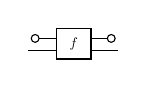
\begin{tikzpicture}[yscale=-1,x=1em,y=1.25em]
    
    \draw [rounded corners] (3,0.25) -- (3.75,0.25);
    \draw [rounded corners] (1.0,0.25) -- (1.75,0.25);
    \draw [] (0.75,0.6) -- (1.75,0.6);
    \draw [] (3,0.6) -- (4,0.6);

    \node[draw, minimum height = 0.5em, minimum width = 1.25em, anchor = west, fill=white] at (1.75,0.4){\scalebox{0.5}{$f$}};
    \node (C1) [draw, circle, fill=white, scale=0.3] at (3.75, 0.25) {};
    \node (C1) [draw, circle, fill=white, scale=0.3] at (1,0.25) {};

\end{tikzpicture}
\end{document}